\documentclass[tikz, multi=tikzpicture, margin=5mm]{standalone}
\usepackage{amsmath}

% --- Colors matching the python script & blog post math ---
\definecolor{Ocol}{HTML}{3273F6}    % Ray Origin (Blue)
\definecolor{Dcol}{HTML}{FF4B4B}    % Ray Direction (Red)
\definecolor{Ccol}{HTML}{109618}    % Sphere Center (Green)
\definecolor{Rcol}{HTML}{990099}    % Radius (Purple)
\definecolor{Acol}{HTML}{FF9900}    % Triangle Vertex A (Orange)
\definecolor{Bcol}{HTML}{0099C6}    % Triangle Vertex B (Light Blue)
\definecolor{Ctri}{HTML}{DD4477}    % Triangle Vertex C (Pink)
\definecolor{Textcol}{HTML}{333333}
\definecolor{Gridcol}{HTML}{E0E0E0}

\usetikzlibrary{calc, intersections, arrows.meta, positioning}

\tikzset{
    >=Stealth,
    font=\sffamily
}

\begin{document}

% ---------------------------------------------------------
% 2. Ray-Sphere 3 Cases (with Roots details)
% ---------------------------------------------------------
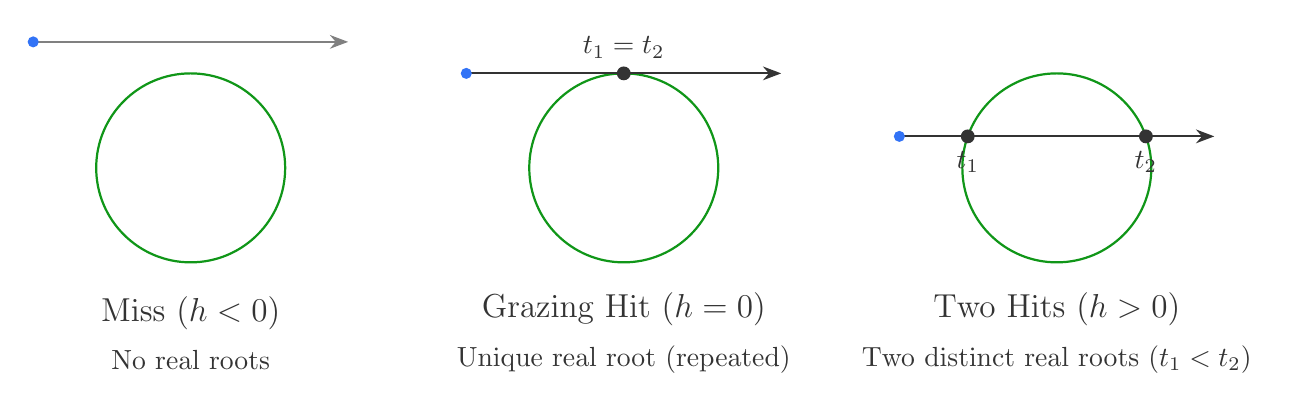
\begin{tikzpicture}[scale=1]
    \def\R{1.2}
    
    % Case 1: Miss (h < 0)
    \begin{scope}[shift={(0,0)}]
        \draw[Ccol, thick] (0,0) circle (\R);
        \draw[->, gray, thick] (-2, 1.6) -- (2, 1.6);
        \fill[Ocol] (-2, 1.6) circle (2pt);
        
        \node[Textcol, font=\large, align=center] at (0,-2.1) {Miss ($h < 0$)\\[0.3em] \normalsize No real roots};
    \end{scope}
    
    % Case 2: Grazing Hit (h = 0)
    \begin{scope}[shift={(5.5,0)}]
        \draw[Ccol, thick] (0,0) circle (\R);
        \draw[->, Textcol, thick] (-2, \R) -- (2, \R);
        \fill[Ocol] (-2, \R) circle (2pt);
        
        % Hit Point
        \fill[Textcol] (0, \R) circle (2.5pt) node[above=2pt, font=\normalsize] {$t_1 = t_2$};
        
        \node[Textcol, font=\large, align=center] at (0,-2.1) {Grazing Hit ($h = 0$)\\[0.3em] \normalsize Unique real root (repeated)};
    \end{scope}

    % Case 3: Two Hits (h > 0)
    \begin{scope}[shift={(11,0)}]
        \draw[Ccol, thick] (0,0) circle (\R);
        \draw[->, Textcol, thick] (-2, 0.4) -- (2, 0.4);
        \fill[Ocol] (-2, 0.4) circle (2pt);
        
        % Intersection calculation
        \pgfmathsetmacro{\xint}{sqrt(\R*\R - 0.4*0.4)}
        
        % Hit Points
        \fill[Textcol] (-\xint, 0.4) circle (2.5pt) node[below=2pt, font=\normalsize] {$t_1$};
        \fill[Textcol] (\xint, 0.4) circle (2.5pt) node[below=2pt, font=\normalsize] {$t_2$};
        
        \node[Textcol, font=\large, align=center] at (0,-2.1) {Two Hits ($h > 0$)\\[0.3em] \normalsize Two distinct real roots ($t_1 < t_2$)};
    \end{scope}
\end{tikzpicture}

\end{document}